\chapter{$\K$ models}
\label{chap:K_model}

\def\Cl{{\text{Cl}^{-}}}
\def\rest{{\text{rest}}}
\def\Erev{{\text{E}_{\text{rev}}}}
\def\KIR{{\text{KIR}}}

In constrat to $\Na$ current which is the result of a single type of $\Na$
channels (inward), $\K$ current is more complex. The $\K$ current is the result
of $\K$ transportation through different types of $\K$-permeated channels that
can be inward or outward.
Due to the many types of $\K$ channels, the nomenclature for $\K$ currents is
quite complicated, and we need to understand them clearly
(Chap.\ref{chap:potassium-channels}).

Even on a single type of excitable cells, there are different types of $\K$
channels \citep{rudy1988duk}. The detail biological phenomenon behind this open
and close of \ce{K+} channel can be referenced from
literature~\citep{yang1995evs,yang1996mbc,french1996ibp,larson1996tms,aggarwal1996css,seoh1996vsr}.

\begin{figure}[hbt]
  \centerline{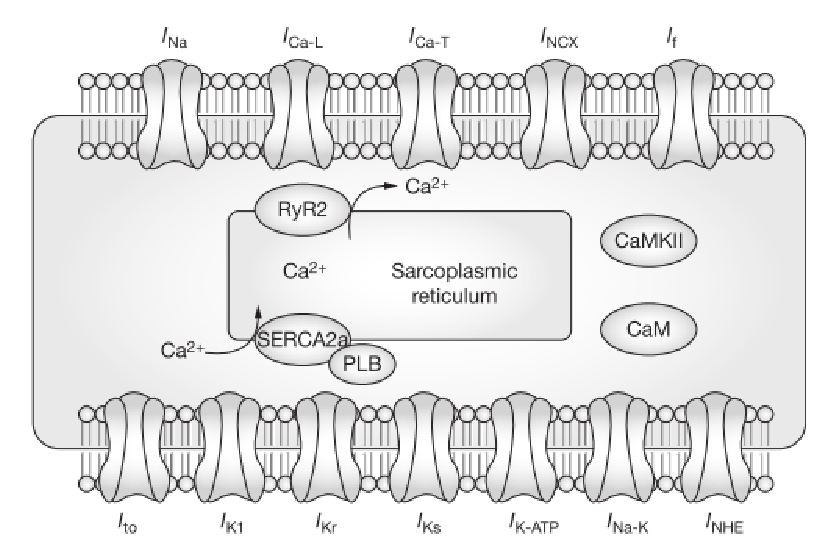
\includegraphics[height=7cm,
    angle=0]{./images/K_channel_all.eps}}
  \caption{Schematic diagram with all K channels on the surface of a cardiac
  cell \citep{nass2008}}
  \label{fig:K_channel_all}
\end{figure}

\section{KDR}
\label{sec:I_Kdr}

This outward delayed-rectifier $\K$ current is $V_m$-dependent and is
responsible for the repolarization of the membrane potential, and thus affecting
AP duration. It contributes to refractory period.

As the channel is activated with a delay, thus giving it the name {\bf delayed
rectifier}. This name was given as the membrane conductance $g_{\ce{K}}$ changes
with a delay after a voltage step~\citep{hodgkin1949icu}. Nowadays, this name is
still being used to denote axon-like K channels even though the current is not
the same as the one used in Hodgkin-Huxley original model; as there are other
$\K$ channels discovered that also change the membrane conductance with a delay
(Sect.\ref{sec:delayed-rectifier}).

The single channel conductance in squid giant axon, lobster membrane and
skeletal muscle is about 15-20pS. In axon, depolarization increases the
frequency of bursts. 

\section{-- Hodgkin-Huxley (1952): $I_\k$ }
\label{sec:KDR-Hogkin-Huxley-1952}

This KDR model in Hodgkin-Huxley model (Sect.\ref{sec:cek+-channel}) is a lumped
of different $\K$ currents. Even this is the main K current, there are also
other K currents to be discusses in the next sections. The second discovered
outward current carring $\K$ ions is A-type $I_A$ current (Connor, Stevens,
1971) - Sect.\ref{sec:A-type-K+current-Connor-Stevens-1971}).

\begin{framed}
The formula in this model can be reused in newer model, but the values should
not, as the 'new' $I_\k$ in newer models ($I_\Kdr$) is different from the old
one. 
\end{framed}

Its kinetics is empirically described by a first-order kinetics $n$ raised to a
power, with/without a first-order of inactivating parameter $k$.
\begin{equation}
  \label{eq:2941}
  g_K = \bar{g_K} \times n^x 
\end{equation}
with $n$ is the activation gating parameter, and $x$ is the Hill coefficient.
{\bf NOTE}: the activating parameter $n$ is raised to a
power to obtain sigmoidity. \textcolor{red}{$\bar{g_K} = 24.31$ m.mho/cm$^2$}.


with
\def\Vhan{{\text{V}_{1/2,\alpha,n}}}
\def\Vhbn{{\text{V}_{1/2,\beta,n}}}
\begin{equation}
  %\label{eq:352}
      \alpha_n = \frac{-0.01 (V_m - \Vhan)}{\exp(-\frac{V_m - \Vhan}{10})-1}
      ,
      \beta_n = 0.125 \exp(-\frac{V_m - \Vhbn}{80})  
\end{equation}
with $\Vhan = -55$ (mV), $\Vhbn = -65$ (mV).

\begin{framed}
NOTE: Even though A-type current is different from KDR, A-type current and
$\Ca$-activated $\K$ current can also produce delayed rectification. 
\end{framed}  

\section{-- Rush-Rinzel (1994)}
\label{sec:KDR-Rush-Rinzel-1994}

Sect.\ref{sec:Rush-Rinzel-1994} developed the KDR model with the same formula as
Hodgkin-Huxley (Sect.\ref{sec:KDR-Hogkin-Huxley-1952})
\begin{equation}
  \label{eq:2941}
  g_K = \bar{g_K}n^4
\end{equation}

with
\def\Vhan{{\text{V}_{1/2,\alpha,n}}}
\def\Vhbn{{\text{V}_{1/2,\beta,n}}}
\begin{equation}
  %\label{eq:352}
      \alpha_n = \frac{-0.01 (V_m - \Vhan)}{\exp(-\frac{V_m - \Vhan}{10})-1}
      ,
      \beta_n = 0.125 \exp(-\frac{V_m - \Vhbn}{80})  
\end{equation}
with $\Vhan = -41$ (mV), $\Vhbn = -51$ (mV).
%%INDEED: Rush-Rinzel uses
%       \alpha_n = \frac{-0.2 (V_m - \Vhan)}{\exp(-\frac{V_m - \Vhan}{10})-1}
%       ,
%       \beta_n = 2.5 \exp(-\frac{V_m - \Vhbn}{80})  
      
\section{A-type K+ current}
\label{sec:A-type-K+-model}

\begin{framed}
NOTE: Even though A-type current is different from KDR, A-type current and
$\Ca$-activated $\K$ current can also produce delayed rectification. 
\end{framed}  

{\bf KNOWLEDGE BASE}: $I_A$ is different $I_K$ (the delayed-rectifier in
Hodgkin-Huxley's work) in several aspects:

\begin{enumerate}

  \item $I_A$ has extremely fast activation (following Vm depolarization), and
  then rapidly inactivate in an exponential fashion (with that maintained Vm
  depolarization), i.e. within 10-100 ms (mostly within 50ms).
  With strong steady-state inactivation, no A-current can be elicited unless the
  membrane potential is conditioned to levels more hyperpolarized than -50mV.
  
 $I_A$ can be described using Hodgkin-Huxley formula  similar to $\Na$ channels.
 Kinetically, A-type currents bear closer resemblance to voltage-gated Na+
 currents than to delayed rectifier K+ currents $I_K$ (or KDR)
 (Sect.\ref{sec:delayed-rectifier}). Even though A-current can reproduce delayed
rectification; the main difference with $I_K$ is that this A-type current
doesn't have $V_m$-dependent bursting behavior (like in neurons). However, in
general, \textcolor{red}{it is often not easy to distinguish A-type current and
``delayed rectifiers''. That's why in cardiac cells, A-type current is also
called delayed-rectifier IK current}.
  
  \item $I_A$ activates at a more hyperpolarized Vm (around -60mV) than that of
  $I_K$ (which activates at around -40mV)
  
  \item $I_A$ is blocked by 4-AP (at high concentration IC50 = 2mM,
  intracellularly applied); and TEA; but compared to $I_K$, $I_A$ is less
  sensitive to TEA.
\end{enumerate}

In particular, they found that a new type of K+ channel in that: {\it the
voltage clamp on the range of membrane potential $> -40$mV in isolated neurone
somas is qualitatively similar to that of squid axon and other neurons. However,
on membrane potential $< -40$mV, e.g.
a step change from -70 mV to -40mV produces a transient outward current which is
much more rapid than the K+ current described in the $> -40$mV range}. This
transient outward, rapidly inactivating current is the result of a different
type of K+ channel; which is called A-type (I$_A$ current, and $g_A$
conductance), and is found to play an important role in repetitive firing.

\textcolor{red}{A-type is a transient outward potassium current}. However, the
term transient outward current has been confusingly used to designate both
\begin{itemize}
  \item  Ca2+-activated K+ currents (elicited by step depolarizations that
  activate large, initial Ca2+ entry events), slowly inactivating,
  voltage-dependent K+currents, and  

  \item true A-type currents (which is rapidly inactivating) and is
  $\Ca$-independent.
\end{itemize}


The current can be fitted  using
\begin{equation}
I = \frac{I_\max}{1+\exp\left( [V_m - V_{1/2}]/k \right)} + \text{baseline}
\end{equation}
with $V_{1/2}$ is the steady-state inactivation midpoints of current
components, $k=RT/(z_\k.F)$. \verb!baseline! is offset current due to 'leak'
current and non-inactivating (Shaw) current present \citep{tsunoda1995}. An
alternate formula was given by
\citep{schutter1986}\footnote{\url{http://www.genesis-sim.org/userdocs/pub-purkinje-deschutter1-conductance1-ka1/pub-purkinje-deschutter1-conductance1-ka1.html}}.
\citep{shibata2000} used a different formula
\begin{equation}
I(t)  = A_0 + A_1 \exp(-t/\tau_1)
\end{equation}
with $A_0$ is the non-inactivating current and the amplitude $A_1$, time
constant $\tau_1$ that best fit the evoked current. To analyze the steady-state
activation, the currents were fit with the following normalized Boltzmann
equation
\begin{equation}
I(V_m) = g_\max \frac{\left( V_m - V_r\right)}{1+\exp\left[ -(V_m-V_{0.5})/k)
\right]}
\end{equation}
with $I(V_m)$ is current (pA) for a given voltage $V_m$ (mV); $V_r$ is the
reversal potential for $\K$ current (about -70mV); $V_{0.5}$ is the membrane
potential for half-activation; $k$ is the slope factor; and $g_\max$ is the
maximal conductance (nS)
\begin{equation}
g = \frac{I}{V_m-V_r}
\end{equation}
To analyze steady-state inactivation, the currents were fit with the following
normalized Boltzmann equation
\begin{equation}
I(V_m) = \frac{I_\max}{1+\exp \left[ -(V_m-V_{0.5})/k\right]}
\end{equation}
with $I_\max$ is the maximal current (pA) to the step $V_m=20$mV measured after
200ms control prepulse -120mV.

\subsection{Single-channel A-current}
\label{sec:single-channel-conductance-A-type-K+-current}
\label{sec:A-type-K+-current-single-channel-conductance}

Single A-current has been described in mammalian sensory neurons (Cooper,
Shrier (1984); Kasai et al. (1986)).

Single A-currents of two different components ($A_1$, and $A_2$) in Drosophila
was described by Aldrich and co-workers (Solc et al. (1987)) with distinct
conductance, voltage-dependency, and gating kinetics.
\begin{itemize}
  
  \item $A_1$ channel is found in myotube (Shaker-gene related -
  Sect.\ref{sec:Shaker-gene}):
  more conductance (12-16 pS), faster and more Vm-dependent macroscopic
  inactivate rate; larger steady-state component; and is less negative
  steady-state inactivation curve the $A_2$.
  
  \item $A_2$ channel is found in neuron: less conductance (5-8 pS); and active
  at lower membrane potential.
\end{itemize}

\subsection{-- K+ currents in MSN}
\label{sec:MSN-K+-currents}

\textcolor{red}{\bf Outward rectifier currents}:
\begin{enumerate}
  \item KDR
  \item KAf
  \item KAs (mature neurons)
  \item non-inactivating current
\end{enumerate}

Early studies in mammalian brain neurons only found $A_2$ type. In the study of
neostriatal neurons, Surmeier (1989) found that two populations of MSN neurons:
one express $A_1$ type ({\it activate at more depolarized potential}); and one
expresses $A_2$ type; but not both.

In Surmeier (1991), he reported a quantitatively change in K+ current by
neostriatal neuron before and after 4-week post-natal development period.
% NOTE: neurons were cultured from either embryos (E15-E19) or pups in their first
% postnatal week; then maintained in culture for 2-days to 6-weeks prior to
% recording
\begin{enumerate}
  \item at near the end of first post-natal week: K+ currents is mainly KAf
  (rapidly inactivating A-current) and very slowly-inactivating delayed
  rectifier K+ current.
  
  A-current is larger; and the only one exhibits inactivation at negative
  membrane potentials.
  
  \item at fourth post-natal week: a third conductance emerge and comes to
  dominate the whole-cell recording in most striatal neurons
\end{enumerate}

\textcolor{red}{\bf Inward rectifier}: Among the two types of inward rectifiers
(KIR, and GKIR), neurons in NAcc only express KIR (Sect.\ref{sec:Kir2.0}). KIR
plays an important role in determining (1) resting membrane potential, (2)
synaptic integration in MSN in both NAcc (Sect.\ref{sec:MSN-in-NAc}) and dorsal
striatum (Sect.\ref{sec:MSN-in-(dorsal)striatum}).

\section{$I_A$: Connor-Stevens-1971}
\label{sec:A-type-K+current-Connor-Stevens-1971}

\citep{connor1971prf} discovered two outward $\K$ currents: $I_K$ and $I_A$ in
gastropod neurone somas. $I_K$ (with conductance $g_K$) is delayed-rectifier
(mapping to Hodgkin-Huxley 1952 model); while $I_A$ is a new type of outward
current. NOTE: More detailed discussion about all kinds of A-type currents is
given in Sect.\ref{sec:A-type-K+current}.

In this study, potassium ions appear to be the predominant current-carrying ion
for $g_A$, its time constants are intermediate between those of $g_\na$, and
$g_K$, and, because it becomes inactivated at above approximately -40 mV, its
predominant role in neurone behaviour is limited to voltages in the subthreshold
range. 
\begin{itemize}
  \item immediately following a spike: $g_K$ dominate neuron's behavior, and
  this current decays toward its resting value
  \item as $g_K$ decrease, $g_A$ is activated and predominates during the middle
  and latter part of the interspike interval.
  
NOTE: the increase of $g_A$ during this phase is important, to counter balance
the inward current via $g_\Na$ and the stimulus current.
\end{itemize}

The rate constants $\alpha_x, \beta_x$ as a function on voltage is represented
here by piecewise linear approximation. \textcolor{red}{NOTE: In their paper,
double subscripts is used: first subscript = the underlying process, i.e. the
gate variable (A,B are used instead of $m,n$), the second subscript = the
channel-type (A-type = new A-type K+ current, K-type = delayed rectifier K+
current, I-type = inward Na+ current)}.







\section{-- KAf ($I_\tof$)}

fast A-type current ($I_\tof, I_\Kr$, ''A'' current) -
Sect.\ref{sec:KAf-current}, is the fast transient $V_m$-dependent $\K$ current.
The channel quickly activates by depolarizing steps from holding potential
negative to the resting potential (as -40mV in molluscan neurons), and then
quickly inactivates \citep{connor1971prf}. The conductance increases with
membrane depolarization. The kinetics is similar to $\Kdr$
\begin{eqnarray}
  \label{eq:2351}
  \bar{g_A}a^4b
\end{eqnarray}
where $a^4$ gives activation with a sigmoid rise and $b$ gives
inactivation with an exponential fall.\begin{equation}
g_A = \bar{g_A}.a^x.k
\end{equation}
This channel is found in several neuronal cells, muscle and eggs with constant
conductance. In atria, Purkinjefibers and subepicardial ventricular cells, the
current denoted as transient outward $\K$ current $I_\to$, gives the
typical ``spike-and-dome'' appearance (the notch). 

In cardiac myocytes, there are two components of $I_\to$: a larger, voltage-activated,
4-AP-sensitive $I_{\to1}$; and a smaller, calcium-activated $I_{\to2}$. In many
cases, they use $I_\to$ as referring to $I_{\to1}$.

The single channel conductance is 15-20pS, without a $V_m$-dependent bursting
behavior. Its main function is to regulate the firing rate, AP repolarization
and latency to the first spike in axon.


\subsection{Campbell et al. (1993) $I_{\to1}$}
\label{sec:campbell93_Ito1}

\citep{Campbell1993} developed models for the $I_{\to1}$ macroscopic current in
ferret right ventricular myocytes which is calcium-insensitive
voltage-dependent. NOTE: The ion selectivity of $I_{\to1}$ in ferret right
ventricular myocytes is consistent with data on isolated rabbit and dog
myocytes; so the model can also be used in cardiac cell models for these
species.

NOTE: In this study, $P_\na/P_\k=0.082$ of $I_{\to1}$ is too small; so it was
assumed that the channel permeate to $\K$ only. Reported from other isolated mammalian cardiac
myocytes, the permeability ratio is higher (0.11-0.26).

\begin{equation}
I_{\to1}= a^3.i.G_{I_{\to1}} (V_m-E_\rev)
\end{equation}
with $G_{I_{\to1}}=68.8$(pS/pF) at 22$^\circ$C; and $E_\rev=(RT/zF)\ln
\frac{0.082[\Na]_o+[\K]_o}{0.082[\Na]_i+[\K]_i}$. 

$a(V,t)$ is the activation gating variable, and $i(V,t)$ is the inactivation
gating variable.
\begin{equation*}
\begin{split}
\frac{da}{dt} &= \alpha_a(V_m)\left[1 - a \right]-\beta_a(V_m).a \\
\alpha_a(V_m) &= 45.16.\exp\left( 0.003577*V_m \right) \\
\beta_a(V_m) &= 98.9 \exp\left( -0.06237*V_m \right)
\end{split}
\end{equation*}
and
\begin{equation}
\begin{split}
\frac{di}{dt} &= \alpha_i(V_m)\left[1 - i \right]-\beta_i (V_m).i \\
\alpha_i(V_m) &= 1.9 \exp\left( \frac{-(V_m+13.5)/11.3}{1+0.051335
\exp\left[-(V_m+13.5)/11.3\right]} \right)
\\
\beta_i(V_m) &= 1.9 \exp\left( \frac{(V_m+13.5)/11.3}{1+0.067083
\exp\left[(V_m+13.5)/11.3\right]} \right)
\end{split}
\end{equation}

For temperature in the range 12-22$^\circ$C, the Q10 is being used as follows
\begin{equation}
\begin{split}
Q_{10}G_{I_{\to1}}=1.84\pm 0.04 \\
Q_{10}\alpha_a(V_m)=3.17\pm 0.54 \\
Q_{10}\beta_i(V_m)=10.62\pm 0.53
\end{split}
\end{equation}


NOTE: The activation has a sigmoid time dependence, which is reproduced by
describing activation as being due to $n$ independent identical activation
gating variables. 

{\bf Single-channel model}: single channel conductance was reported previously,
with 14pS (rabbit atrium, [K]$_p$=5mM) and 19.9pS (rabbit AV node,
$[\K]_p=5.4$mM); 27pS and 5pS (mouse ventricular myocytes, $[\K]_p=5.4$mM). In
this study (ferret right ventricular myocyte), the single channel conductance
was 4-7pS ($[\K]_p=5.4$mM). The differences here can be due to experimental
factors, or species variant. In {\it Drosophila} myotube A$_1$-type $\K$
channel, the conductance was in the range 12-16pS ($[\K]_p=2$mM), and A$_2$-type
$\K$ channel has the conductance in the range 5-8pS ($[\K]_p=2$mM).


\begin{framed}
4-AP has been used as pharmacological tools for the study and
classification of $\K$ channels in various tissues. 4-AP is used as an
indicator to identify the voltage-dependent inactivating $I_\to$ (or
$I_\text{A}$) $\K$ currents. Also, in mammalian cardiac myocytes, 4-AP is used
to separate $I_\to$ into 2 different components: $I_{\to1}$ and $I_{\to2}$. 
\end{framed}


\citep{Campbell1993b} developed models incorporating [4-AP], focusing
on $I_{\to1}$ $\K$ channels which is 4-AP-blockable. The mechanism of block by
4-AP is 4-AP-level dependency. However, the block is incomplete, even at [4-AP]=10mM;
and the mechanism of block is complex (see below), with voltage- and
frequency-dependent characteristics. The degree of block is lessened with either
increasing frequency or depolarization.

At [4-AP]=5mM, it not only reduces peak $I_{\to1}$, but also slowed the
activation and time-course of current decay, Fig.\ref{fig:Ito1_4-AP}(A); and the
peak $I_{\to1}$ is a sigmoidal function of [4-AP] (mM), fitted by the smooth
curve to a single-binding site equation.
\begin{equation}
\frac{I_{\to1,\text{4-AP}}}{I_{\to1},\text{control}} =
\frac{1}{1+\frac{[4-AP]}{K_d}}
\end{equation}
with $K_d = 0.201$ (mM) (which is independent of $V_m$, with value before 
correction for the leak current is $K_d=0.191\pm 0.011$mM)
(Fig.\ref{fig:Ito1_4-AP}(B)).

The results also showed that the for a given [4-AP], the peak is independent of
the pulse potential over the range (from +20 to +100mV with 10mV increment) at
which $I_{\to1}$ is activated (and holding potential -70mV); yet it's dependent
on the holding potential. The protocol was also repeated with increasing [4-AP]
(from 0.0625mM-10mM). At higher [4-AP] ($>1$mM), the pulse frequency was
increased (one pulse per 10-30s), while at lower [4-AP], one pulse per 1-2min.

\begin{figure}[hbt]
 \centerline{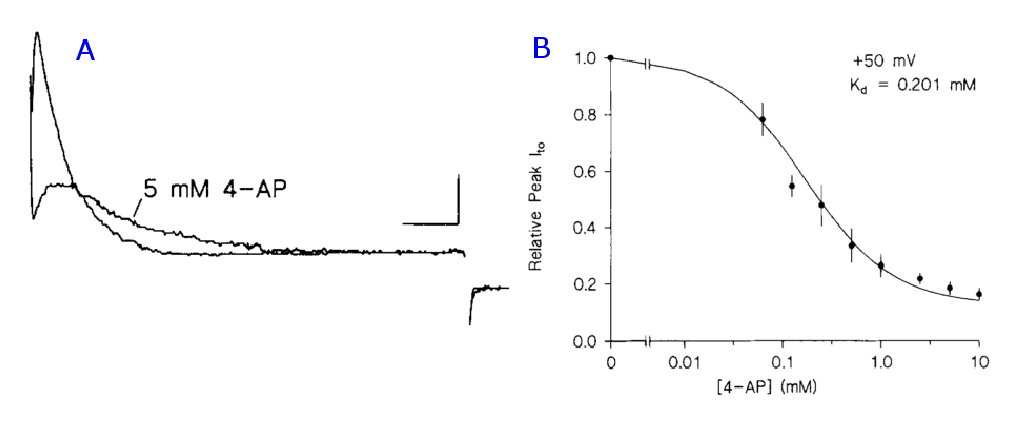
\includegraphics[height=5cm, angle=0]{./images/Ito1_4-AP_campbell93.eps}}
\caption{(A) At 800ms V-clamp pulses of +50mV (holding potential Vm=-70mV) and
5mM 4-AP (calibration: 100ms, 100pA); (B) Dose-reponse curve for
block of peak $I_{\to1}$ by 4-AP \citep{Campbell1993}}
\label{fig:Ito1_4-AP}
\end{figure}

Some other studies suggested 4-AP could not bind to the channels while the
channels are in their resting state (i.e. tonic block could not develop at
hyperpolarized potentials.). However, in this study, they showed that the
channels don't have to be previously activated in the presence of 4-AP for the
block to develop. So, they suggested that 4-AP bind to the closed
(resting) state, but doesn't bind significantly to the inactivated states. Thus,
they suggested the channels have two non-conducting states: C and I. 

Tonic block is prevented at 0mV; which indicates that no substantial binding
occurs to states I1 and I2 in model-1 and state I1 in model 3. The two models
differ only in the inactivation; while the activation sequences are the same
(C3,C2, C1, O). As 4-AP only bind to the channel at the activating sequence, and
single-binding site is assumed, there are three possible cases, with $B_n$
denotes 4-AP-bound closed state.

However, a more complex multiple-closed state binding model is required,
Fig.\ref{fig:Ito1_4-AP_campbell93_model}. There are alway ambiguities in
assignment the rate constants to specific transitions between closed states \citep{hille1992mb}.


\begin{figure}[hbt]
 \centerline{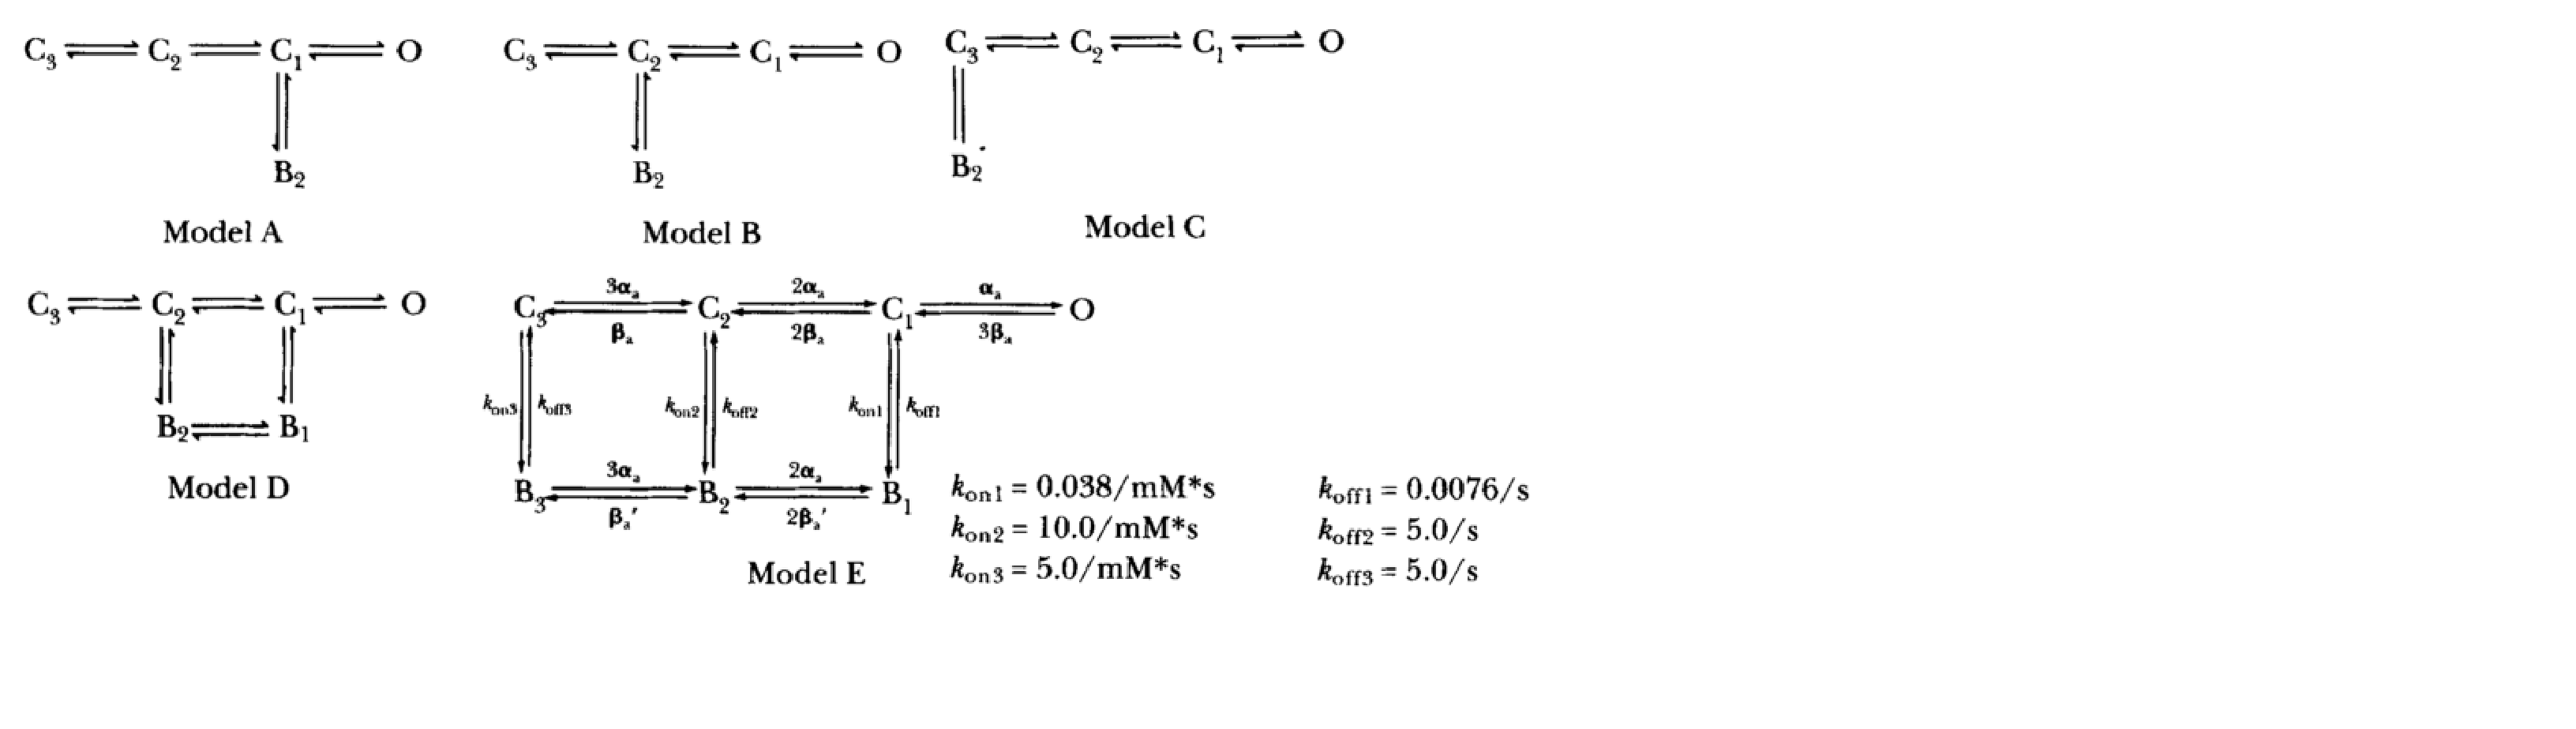
\includegraphics[height=5cm, angle=0]{./images/Ito1_4-AP_campbell93_model.eps}}
\caption{Different proposed models of $I_{\to1}$ that incorporate 4-AP binding
\citep{Campbell1993}}
\label{fig:Ito1_4-AP_campbell93_model}
\end{figure}


\subsection{Greenstein et al. ($\Ito$)}
\label{sec:Greenstein_Ito1}

$\Ito$ is the $\Vm$-dependent $\Ca$-indepenent current that play an important
role in shaping the early phase of cardiac ventricular AP (the notch). It's an
transient outward current. However, the role of $\Ito$ to APD is unclear. In
failing hearts, the expression levels of genes to encode for $\K$ decrease. 

In canine and human, $\Ito$ is likely a combination of Kv4.3 and Kv1.4-enoded
currents ($\Ikvft, \Ikvof$). 

\begin{equation}
\Ikvof = \frac{P_\Ikvof}{\Csc} \frac{F^2V_m}{RT} \Po(V_m,t)
\frac{[\K]_i-[\K]_o\exp(-V_mF/(RT))}{1-\exp(-V_mF/(RT))}
\end{equation}
with $P_\Ikvof$ is maximum channel permeability,
$\Csc=10^4$pF/mm$^2$=1$\mu$F/cm$^2$ is the specific membrane capacity; and $\Po$
is the probability of channel opening. 

\subsection{Korngreen et al. (2000) - Pyramidal L5 neuron}

\citep{korngreen2000}


\section{Kv1.2}

It has been found in 
\begin{enumerate}
  \item MSN : Sect.\ref{sec:Kv1.2-Shen2003-MSN}

This slowly inactivating, low-threshold K+ current has been implicated in the
regulation of state transitions and repetitive activity in striatal medium spiny
neurons. This channel opens in a subthreshold voltage range but unlike Kv4
channels inactivates slowly.

  \item 
\end{enumerate}

\subsection{Shen et al. (2003) - MSN}
\label{sec:Kv1.2-Shen2003-MSN}

Using different blockers, the result showed that the Kv current
(Sect.\ref{sec:Kv1-channels}) only affected by Kv1.2 blockers; and is not
affected by Kv1.1 or Kv1.6 blocker \citep{shen2003}.

Channel gating was assumed to conform to a Hodgkin-Huxley-like formalism
\begin{equation}
\begin{split}
I = \bar{G_\max} \times m^2 \times \left[ a * h + (1 - a) \right] \times \left(
\Vm - E_\rev \right)  \\
\tau_m = \tau_{m,0} + C_m \exp \left( - \frac{\Vm -
V_{\tau_m}}{V_{\tau_{Cm}}} \right) \\
\tau_h = \frac{C_h}{\alpha \exp( \frac{\Vm - V_{\tau_h,1}}{V_{\tau_{c,1}}}) 
                    +\alpha \exp( \frac{\Vm - V_{\tau_h,2}}{V_{\tau_{c,2}}}) }
\end{split}
\end{equation}
with $a $ represent the fraction of channel always inactivate.


\begin{verbatim}
Vmh = -27 mV; Vmc = -16 mV;
tau_m0 = 3.4 ms; Cm = 89.2; Vtau_hm = 34.3 mV; Vtau_cm = 30.1 mV; for
the inactivation process, the parameters were: Vhh = -33.5 mV;
Vhc = 21.5 mV; Ch = 548.7; Vtau_h1 = -0.96 mV; Vtau_c1 = 29.01 mV;
Vtau_h2 = -0.96 mV; Vtau_c2 = 100 mV.
\end{verbatim}
Temperature correction: Q10 = 2.3 (or $\Phi$=3 for conversion from 22 to 35
degree Celcius).


\section{Kv4 (A-type)}


In granulle cells: midpoints of activation (Vhact of -4.6 mV) and inactivation
(Vhinac of -42.2 mV) and the slope factors (kact of 5.0 mV and
kinac of 5.7 mV).  (Shibata et al., 2000)

The IA took more than 40 msec to fully recover from inactivation at -120 mV, and
the value of $\tau$ (recovery time constant) was 6.6 msec at -120 mV, 15.5 msec
at -80 mV, and 41.4 msec at -50 mV.

The amplitude of mKv4.2 currents was 713.9 $\pm$ 80.5 pA/pF at +40 mV.



\section{Shaker $K_v$ current}	


\citep{zagotta1994}


\section{KIR}
\label{sec:KIR-models}

The KIR current is sensitive to extracellular potassium concentration,
and the steady-state curve was therefore shifted to match the given [K+]$_o$,
and and potassium reversal potential.

\subsection{Kinetics of an inward-rectifier current}
\label{sec:Kir-channel-kinetics}

All $\Kir$ requires PIP2 for activation (Sect.\ref{sec:PIP2}).
They are regulated by several mechanisms (oxygen tension, pH, G-proteins, ATP,
etc.) and some are $V_m$-gated (Sect.\ref{sec:Kchannel_Vm-dependent}). 

A $\K$ channel that is {\bf inwardly-rectifying} ($I_\Kir$) if, at any given
driving force ($\Vm-E_\rev$), it passes current (positive charge of $\K$) more
easily and of greater magnitude in the inward direction (into the cell), than
the outward direction (out of the cell), i.e. depolarizing the membrane. The
inward current is shown as negative current (downward deflection).

\begin{mdframed}
Unlike Kv channels (which are activated by depolarisation, allowing the outward
flow of K+ in depolarised cells), Kir channels on the other hand, preferentially
conduct K ions in the inward direction, from the extracellular fluid into the
cell. 

Upon membrane depolarization, i.e. $(\Vm-\Erev)>0$, the pore of these Kir
channels becomes blocked by positively charged Mg2+ or polyamine molecules,
leading to the rectification of current flow which gives this channel sub-family
their name. Kir channels stabilise the membrane potential once it approaches the
K+ equilibrium potential, which is expected to regulate cell's resting membrane
potential (Sect.\ref{sec:resting-potential}).

\end{mdframed}

Suppose $\Erev$ is the reversal potential of $\K$ channel
(Sect.\ref{sec:reversal-potential}), then the inwardly rectifying $\K$ channels
behave:
\begin{enumerate}
  \item If $\Vm < \Erev(K)$ (i.e. at hyperpolarized potential below $E_K$): the
  channels are unblocked (from internal $\Mg$), allow the channel to open with
  significant inward $\K$ influx.
  
  Kir support the flow of positively charged K+ ionsinto the cell, pushing the
  membrane potential back to the resting potential $\Erev$.
  
  $I=g(\Vm-\Erev)$ is negative
  
  \item If $\Vm > \Erev$ (when membrane potential is positive to $E_K$): the
  channel is blocked by internal $\Mg$ and polyamines, i.e. no $\K$ current via
  the channel.
\end{enumerate}

An example is showed in Fig.\ref{fig:rectifier_current} which display whole-cell
recording of Kir2.x expressed in HEK293 cell (Sect.\ref{sec:HEK293-cell}). {\bf
IMPORTANT}: The voltage number is indeed $(\Vm - \Erev)$, i.e. the relative of
$\Vm$ w.r.t. to the reversal potential of the Kir2.x channel. If we plot the
peak current vs. $\Vm$, i.e. I-V curve, then the result looks like
Fig.\ref{fig:Kir_current}.

\begin{figure}[hbt]
 \centerline{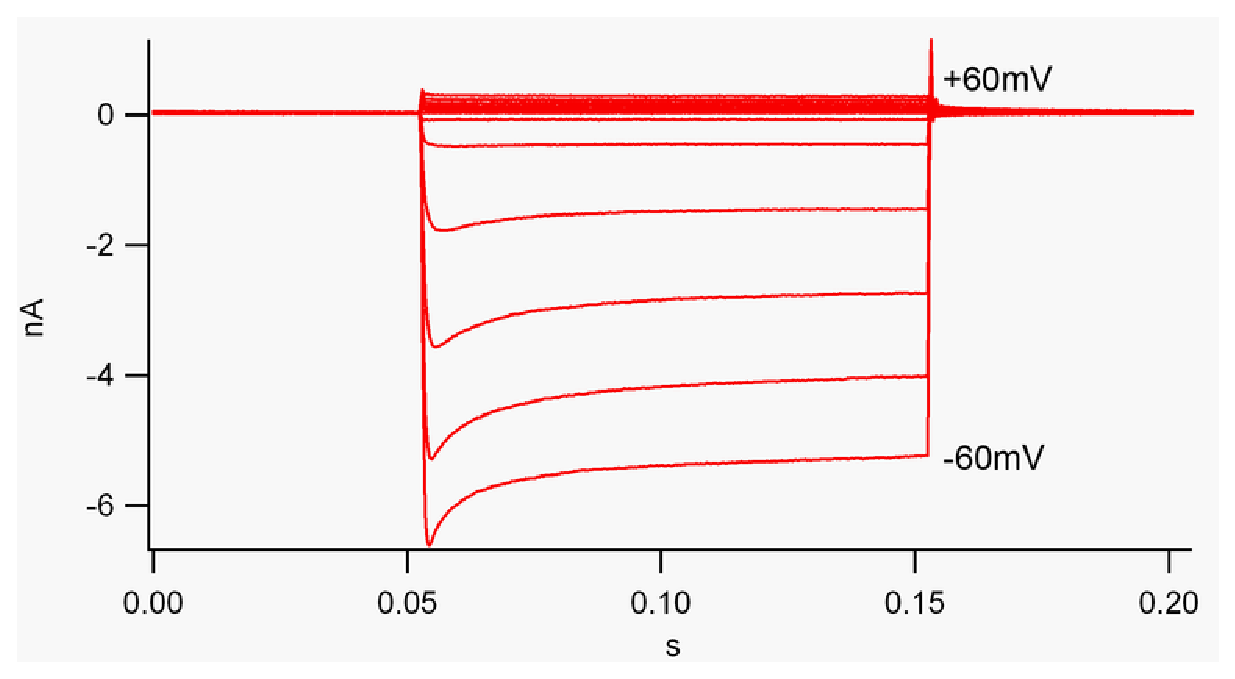
\includegraphics[height=5cm, angle=0]{./images/inward_current.eps}}
\caption{ The whole-cell voltage clamp in HEK293 cell evoked inward
potassium-selective currents which rapidly reached a peak amplitude and then
relaxed to a steady-state level. This is Kir2.x channel. \textcolor{red}{The
values of voltages traces is the value of} $(\Vm - \Erev)$. 13 responses
superimposed in the image using Voltage-clamp (top is 
$(\Vm -E_{\rev,\K}) = +60 $mV , bottom is $(\Vm - E_{\rev,\K}) = -60$mV).
The channel display strong inward current at negative potential, and 
then reduce upon depolarization. At strong positive potential, it can display
small (positive) outward current. \textcolor{red}{This is an example of a
strong inward-current, as the outward current is very small even when $\Vm$ is
very positive to $\Erev$}}
\label{fig:rectifier_current}
\end{figure}


\begin{figure}[hbt]
  \centerline{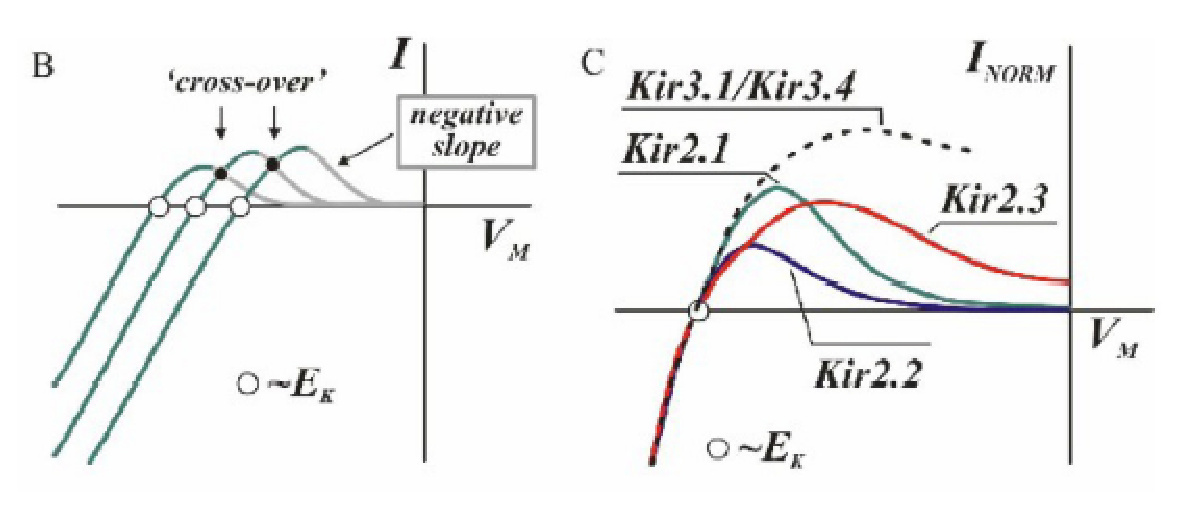
\includegraphics[height=5cm,
    angle=0]{./images/Kir_current.eps}}
  \caption{{\bf (B)}. When $\Vm$ is negative to $\Erev(K+)$, the inward current
  becomes stronger. When $\Vm$ is positive to $\Erev(K+)$, it may display an outward
  behavior. This outward currents of $\Kir$ current (conductance) increases and
  after a certain membrane potential, it declines upon further depolarization
  and thus exhibits a characteristic region of so-called {\it negative slope}
conductance. Another unique property is the dependence upon extracellular
$[\K]_o$. The increase in $[\K]_o$ shifts the $\Kir$ current/voltage
relationship nearly in parallel with the reversal potential $E_\K$, leading to a
{\bf ``crossover''} phenomenon, i.e. at potential positive to the
crossover, the $\Kir$ conductance increases rather than decreases.
~\citep{Anumonwo2010}. {\bf (C)} The different conductances shape at
inward-stage betwen Kir2.1, Kir3.1/Kir3.4, Kir2.3 and Kir2.2}
\label{fig:Kir_current}
\end{figure}


Inward-rectifier current helps resisting $\K$ efflux at positive potentials. The
inward current is active at hyperpolarized potential, and decreases under
depolarization. Thus, the inward rectification results in no detectable outward
current via these channels at plateau-range potentials. After the membrane has
repolarized (from the peak +40mV) to -20mV, then the inward rectifier again
begin to conduct outward current. As the membrane continue to repolarize to its
resting level, the current dominates the net outward conductance.
  
Inward rectification is an important property of cardiac, skeletal muscles and
neurons.  This is the channel that provides resting conductance in some cells,
as it dominates the outward current at resting potential. The channel involves
in cardiac pacemaker activity, egg fertilization, and regulating of fire
frequency in axons.

\subsection{KIR (Hagiwara, Takahashi (1974, 1980)) - starfish egg cell}
\label{sec:KIR-model-Hagiwara-Takahashi-1974-starfish-egg-cell}

The KIR in immature egg cell membrane of a starfish {\it Nordora punctiformis}
was modeled with the conductance that is a function of $\Vm$ and a function of
$[\K]_o$. Hagiwara, Takahashi (1974) examined the current by varying $[\K]_o$
and $\Vm$. They found that the curve change in parallel with changing $E_\K$,
Fig.\ref{fig:Kir_current}.
\begin{equation}
g_\k = f(\Vm, [\K]_o, t)
\end{equation}

The voltage-dependent part is represented using Boltzmann function:
$1/(1+\exp(V-Vh)/k))$. The slope of $\log I_\KIR - \log[\K]_o$ line for a fixed
$\Vm$ is approximatedly 1/2 indicates that the current is proportional to the
square root of $[\K]_o$.

\begin{equation}
g_K = A \left[  1 + \exp\left( \frac{\Vm - V_h}{k_h} \right) \right]^{-1}
\left([\K]_o\right)^{1/2}
\end{equation}
with $V_h= V_\rest - 15$ (mV); and $k_h = 7$ (mV). 

The permeability ratio $P_x/P_\k$ of ions through KIR: \ce{T1^+}(1.5) > K(1.0) >
Rb (0.3 to 0.4) > \ce{NH4} (0.03 to 0.04) > Na, Cs. 

\textcolor{red}{Q10}: The temperature dependency was Q10 = 1.62 (Hagiwara \&
Yoshii, 1980).


\subsection{KIR (Leech, Stanfield (1981)) - skeletal muscle}
\label{sec:KIR-model-Leech_Stanfield-1981-skeletal-muscle}


Leech and Stanfield (1981) studied KIR by varying $[\K]_i$, instead of $[\K]_o$.
REMEMBER: When changing $[\K]_o$, the conductance shift along the potential axis
(i.e. the change in location of activation curve), Fig.\ref{fig:Kir_current}.
However, when $[\K]_i$ is changed, with a given $[\K]_o$, the conductance does
not shift. Instead, $g_\k$ is relatively higher at $\Vm=E_k$ if $E_\k$ has been
made more negative by raising $[\K]_i$; and relatively smaller at $E_\k$ if
$E_\k$ has been made more positive by reducing $[\K]_i$.

{\bf SUMMARY}: The relation of $g_k$ of KIR is better described as a function of
$\Vm$ and $[\K]_o$; rather than $(\Vm - E_\k)$.
\begin{equation}
g_\k = f(\Vm, [\K]_o, t)
\end{equation}
with the ratio of  $I_o$ (initial current); $I_s$ (steady-state current,
measured at after 2 second)

\begin{equation}
I_o/I_s = 0.57 \frac{1}{1 + \exp \left( (\Vm-V_h)/k_h \right) + 0.43}
\end{equation}
with
\begin{itemize}
  \item $V_h$ = - 11 (mV); $k_h = 7.5 $(mV) for 160 mM $[\K]_o$
  
  \item $V_h$ = - 19.5 (mV); $k_h = 7.5 $(mV) for 80 mM $[\K]_o$
  
  \item $V_h$ = - 36.5 (mV); $k_h = 7.5 $(mV) for 40 mM $[\K]_o$
   
\end{itemize}


It can be explained by the two-state model
\begin{equation}
\text{Close/Low-conductance} \ce{<=>[\alpha_n][\beta_n]} \text{Open}
\end{equation}
with 
\begin{itemize}
  \item $\alpha_n$ is a rate constant for opening and depends steeply on voltage
  $\Vm$
  
  \item $\beta_n$ is a rate constant for closing and is relatively independent
  of potential
\end{itemize}


\subsection{KIR (Nisenbaum, Wilson (1995)) - dorsal striatum}
\label{sec:KIR-model-Nisenbaum-Wilson-neostriatum-neuron}

They create a simple model to study the balance between inward-rectifying and
outward-rectifying currents.

\textcolor{red}{Inward-rectifying current}: The Bolzmann equaiton is used
\begin{equation}
g = \bar{g} \times \left( 1 - \frac{1}{1+ \exp\left( (\Vm - V_h)/k_h \right)} 
\right)
\end{equation}
with $\Vm$ is membrane potential, $V_h$ is half-activation voltage 
($V_h=(E_\k - 15)$ mV); $k_h = 10$ (mV).

Consider 3 values of $E_\k$
\begin{enumerate}
  \item $E_\k=$-70 (mV); so $V_h = -85 $(mV)
  
  \item $E_\k=$-90 (mV); so $V_h = -105 $(mV)
  
  \item $E_\k=$-110 (mV); so $V_h = -125 $(mV)
\end{enumerate}

\textcolor{red}{Outward-rectifying current}: The Bolzmann equaiton is used
\begin{equation}
g = \bar{g} \times \left( \frac{1}{1+ \exp\left( (\Vm - V_h)/k_h \right)} 
\right)
\end{equation}
with $V_h = -60$(mV); and $k_h = 10$(mV).


\subsection{KIR - IRK1 (Mermelstein, Surmeier (1998)) - nucleus accumbens}
\label{sec:KIR-model-Mermelstein-Surmeier-1998-NAc}



\subsection{KIR2 (Kubo - Murata, 2001)}

The steady-state activation curve was fitted to a mouse KIR channel composed of
KIR2.1 subunits expressed in human embryonic kidney cells. The steady-state
curve is then shifted to match the $[\K]_o$ and $E_\k$ in rat.



\section{IKr - Clancy(2001)}

\citep{clancy2001}

\section{IKs - Silva(2005)}

\citep{silva2005} 
 
 \section{Ito - Bondarenko (2004) - mouse (25$^\circ$C)}
 
 \citep{bondarenko2004cma}
 
 \section{BK(Ca) - Shao et al. (1999)}
 
 The big conductance $\Ca$-dependent $V_m$-gated $\K$ current (BK(Ca)) is
 described in Sect.\ref{sec:BK-current}.
 As the current needs to be activated first by $V_m$, before it can be modulated
 by $[\Ca]_i$, typically three states are used: Close, Open, and Inactivated.
\begin{verbatim}
C  <=> O -> I -> C
\end{verbatim}
This is a model for BK(Ca) $\alpha$-a generic $beta$ auxiliary subunit.

\section{SK(Ca) - Moczydlowski (1993)}
\label{sec:SK(Ca)-Moczydlowski-1993}

SK(Ca) is discussed in Sect.\ref{sec:SK_current}.
The gating behavior is derived from single-channel recording extracted from rat
skeletal muscle incorporated into planar phospholipid bilayer.
The kinetics is Voltage-independent (-60 mV to +60mV), Ca2+-dependent (tested
with 0.1$\muM$ - 10$\muM$) (based on first-order rate constants).
They aimed to develop a kinetic model able to predict both the microscopic and
macroscopic behavior of the channel.
% \textcolor{red}{The unitary conductance is 290$\pm 30$ pS, which map to that
% of BK current, so not sure if this is an SK(Ca) or not.?}

The unitary current about 20 pA (Fig. 2).
Total event: 200-1000 opening for 20 second of channel time.
Time resolution (0.25ms - 1ms). NOTE: slow closure, i.e. closing events lasting
longer than 500 ms, were excluded from the present analysis.

Rare substate conductance level of -50\% of the full open state, lasting as
long as 50 ms in duration is also observed. The frequency of occurence of
substate events did not appear to vary with voltage and $\Ca$ concentration.

NOTE: Both rate substate and slow closure does not affect the analysis due to
the rare occurence of them.

REMIND: A more serious problem that could affect our analysis of channel gating
was variation in the Ca" concentration dependence and voltage dependence from
channel to channel.

\subsection{Analysis}

Model is built from 72 combination of Vm and $[\Ca]_i$.
They measure the mean open time and closed time (Sect.\ref{sec:mean-open-time}).

From observation of the single-channel recording data, there are two types of
close events:
\begin{itemize}
  \item well-resolved closed-state events: about 37\% of the population, and
  mean-time 16ms
  
  \item short-lived clustered spikes (flickers) emanating from open-state
  level in a bursting pattern: about 63\% of close-event population, and
  mean-time $< 0.4$ (ms).
\end{itemize}
channel spends only a small fraction of the
total time in flicker events .

SUGGEST MODEL
\begin{verbatim}
C <=> C2 <=[fast-kinetic]=> O1 <=> O2
           for short-lived
           spikes
\end{verbatim}


Removing these short-lived closed and open events ($< 1$ ms): 
\begin{itemize}
  
  \item the dwell-time in close event can be fitted with a single exponential
  (represented by a single straight line) Fig. 4(B) upper trace with $\tau_C=16$ ms
  
  \item the dwell-time in open event can be fitted with a single exponential
  (reprsented by a single straight line) Fig. 4(B) upper trace with $\tau_O =18$
  ms 
\end{itemize}
They refer to this residual gating pattern as the primary gating mode, since the
channel spends >97\% of total time in.
This effectively restrict the analysis to conditions in which the
overall mean closed time is $>3$ ms.

\subsection{Model}

Mean open dwell-time (Sect.\ref{sec:dwell-time-mean}) is plotted vs $[\Ca]_i$;
and mean closed dwell-time is plotted vs reciprocal of $[\Ca]_i$
\begin{itemize}
  \item $\tau_O$ is a linear function of $[\Ca]_i$
  
\begin{equation}
\tau_O = \frac{1 + [\Ca]/K_4} \times 1/\alpha
\end{equation}  
  \item $\tau_C$ is a linear function of $1/[\Ca]_i$


\begin{equation}
\tau_C = \frac{1 + K_1/[\Ca]} \times 1/\beta
\end{equation}  
\end{itemize}
to hold over the range of open-state probabilities of 0 .05-0 .95.

Even though the mean dwell-time $\tau_O$ and $\tau_C$ also show $V_m$
dependency; this tends to converge to the same value 
\begin{itemize}
  \item value 1  = $1/\alpha$: at low $[\Ca]_i$, and for all different values of
  $V_m$

  \item value 2: at high $[\Ca]_i$, and for all different values of $V_m$
\end{itemize}


\subsection{General model: 8-state}


Using log-log plot of $K_\eq$ vs. $[\Ca]_i$:
The slope of the Hill plots of open-closed equilbrium (log($P_O/(1-P_O)$)
vs. $[\Ca]$ (log([Ca]/M)) is greater than 1; suggesting there is more than 1
binding site (Fig.11 C)
\begin{itemize}
  \item slope 1.2 at negative voltage
  \item slope 1.8 at positive voltage
\end{itemize}

General model: 8 states
\begin{itemize}
  \item 4 close states: zero conductance
  \item 4 open states: same conductance value
\end{itemize}

\begin{figure}[hbt]
 \centerline{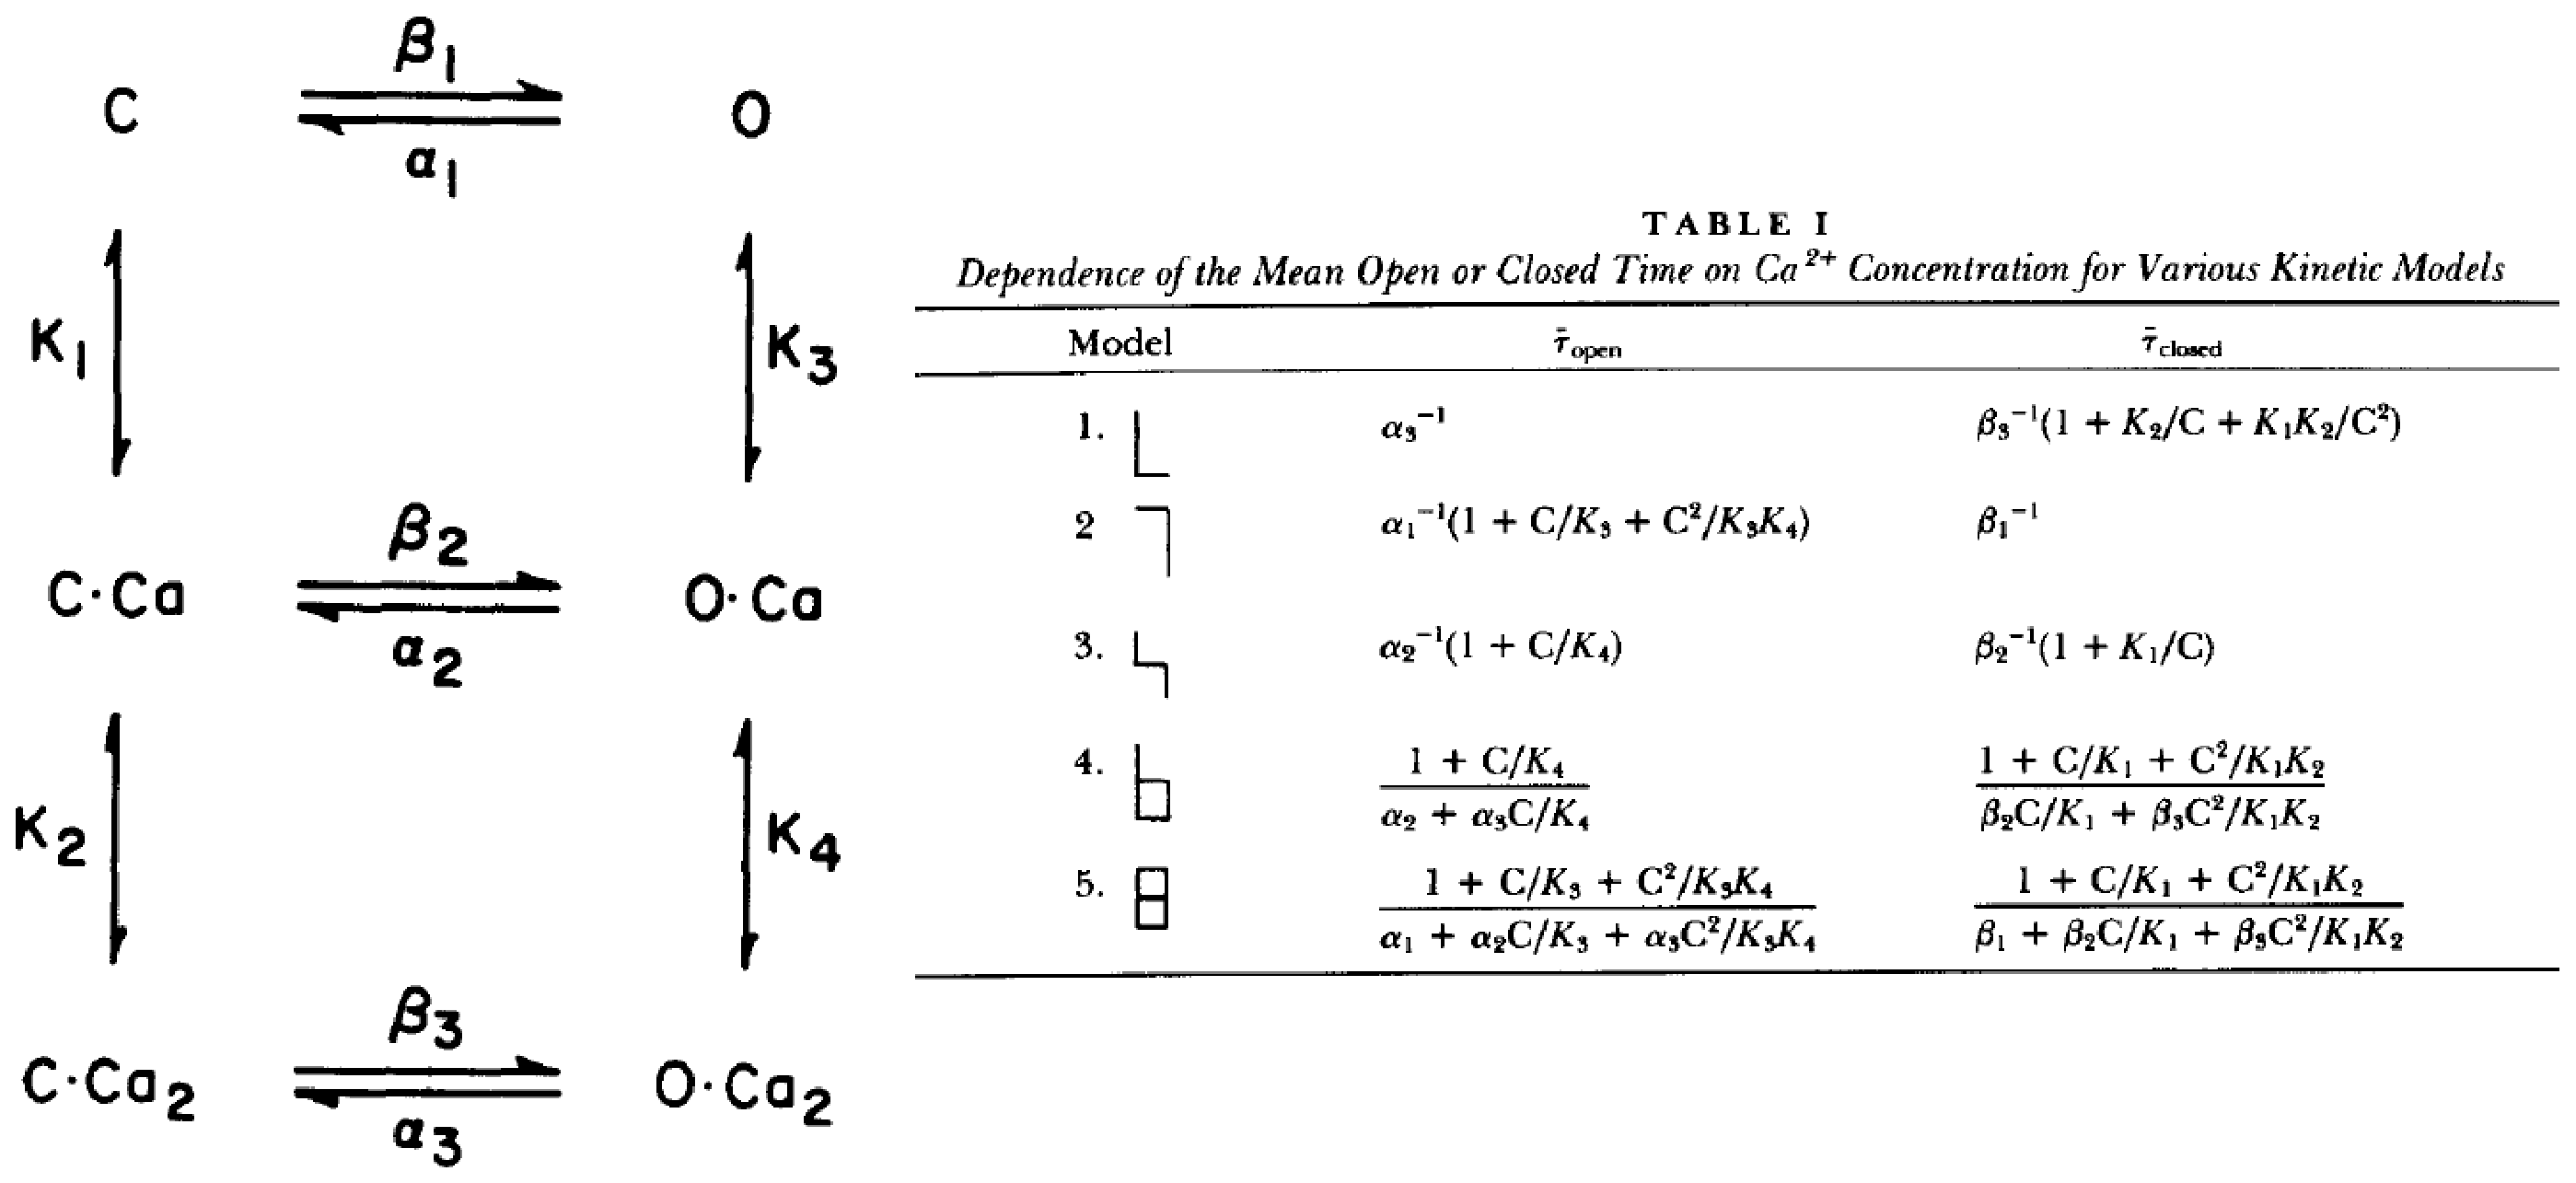
\includegraphics[height=5cm]{./images/SK(Ca)-model.eps}}
\caption{A general 8-state scheme: first-order transitions between C and O with
reverse rate constant $\alpha$ and $\beta$; while transition between close
states (or between open states) are modeled as fast equilibrium with 4
dissociation constants: K1, K2, K3 and K4.
Table 1: subset pathways (C=[$\Ca$]). For microscopic reversibility:
$K_1\beta_1/\alpha_2 = K_3\beta_1/\alpha_1$ (upper), and $K_2\beta_2/\alpha_3= K_4\beta_3/\alpha_2$ (lower)}
\label{fig:SK(Ca)-model}
\end{figure}

\subsection{Scheme R1: 4-state}

IMPORTANT: it is possible that the probabilities for some of the states are
small under normal conditions, so that we can effectively ignore them .
We then try different possible subset pathways,
Fig.\ref{fig:SK(Ca)-model}(Table 1).
\textcolor{red}{Only model 3 is reasonable as it shows the open time constants
as a linear function of [Ca] and close time constant is a linear function of
1/[Ca]}.

\begin{equation}
\ce{C <=>[k_1\text{[Ca]}][k_{-1}] C.Ca <=>[\beta][\alpha] O.Ca
<=>[k_4\text{[Ca]}][k_{-4}] O.Ca_2}
\end{equation}
with $K_1 = k_{-1}/k_1; K_4 = k_{-4}/k_4$.
NOTE: $\beta=\beta_2$, $\alpha=\alpha_2$.


\textcolor{red}{HOW TO FIND} $\alpha, \beta$, $K_1, K_4$?
\begin{enumerate}
  \item analyze the slope and intercept of the straight lines in the data above

plot for $\tau_o$ vs. [Ca]: intercept at $1/\alpha$, slope $1/(\alpha K_4)$

plot for $\tau_c$ vs. [Ca]: intercept at $1/\beta$, slope $1/(\beta K_1)$

\end{enumerate}

As all the straight lines converge at points closed to the y-axis, i.e.
the intercept is not a strong function of voltage, and can be estimated
as: ($\alpha=280$ (1/s) and $\beta=480$ (1/s)).

However, the slopes are strong functions of voltage, expressed inside $K_1$ and
$K_4$, (data in Fig.10) which can be fit well with a single exponential function
for the case of ionic channel blocker
\begin{equation}
K(V) = K(0)	 \times \exp\left(-z\delta FV/(RT)\right)
\end{equation}
with $K(0)$ is zero-voltage dissociation constant, $z$=valence of $\Ca$ (+2),
$\delta	=$ fractional distance of the electric field that is felt by the ion

\begin{mdframed}

HYPOTHESIS to explain $V_m$-dependent of Ca2+ binding: 
First, a conventional interpretation implies these binding sites are located in
an electric field, represented by the value $\delta$. The derived value $\delta$
of 0.75 and 0.95 tells that the location of the sites is deep in the electric
field.
\begin{itemize}
  \item hypothesis 1: possible locations at the mouth of the channel ({\it cis}
  side) - unattractive due to repulsive force exerted by two divalent ions $\Ca$
  and one monovalent ion $\K$ crowded together in a small area, i.e. at least 5
  negative charges distributed throughout the site to prevent the mutual
  repulsion which still possible if the 'wide mouth' of the channel.
  
  \item hypothesis 2:  $\Ca$ activation site is far away from conduction pathway
  (channel pore), but is more sensitive to $V_m$ as it is closer to the lipid
  membrane (lipid head groups)

  \item hypothesis 3: actual $\Ca$ binding rates are voltage-independent; yet
  voltage can lead to the change in protein structure making the binding easier,
  i.e.  the coupling between voltage and apparent $\Ca$ binding affinity rather
  than a direct influence of the electric field on the movement of $\Ca$ ions.

\end{itemize}

\end{mdframed}


\begin{itemize}
  \item since $K_1 > K_4$ : $\Ca$ binding to close state exhibit lower affinity
  than binding to open state 
  
  \item the difference in affinity also enhanced at higher voltage: this can be
  explained by the difference in $\delta $ value for the two binding reactions.
  
  low-affinity site is located at 70-80\% of electric field (i.e.
  $\delta =  0.67-0.84$), while high-affinity site is located at 90-100\% of
  electric field (i.e. $\delta = 0.9-1.0$)
\end{itemize}

Opening probability $P_o$, was measured as the simple fraction of time in the
equilibrium open state at various Ca2+ concentrations and voltages, i.e. can be
derived from equilibrium treatment of the scheme above
\begin{equation}
P_o ([\Ca],V_m) = \frac{[\ca]^2 + [\ca] K_4}{[\ca]^2 + [\ca]K_4
(1+\alpha/\beta) + K_1 K_4 (\alpha/\beta)}
\end{equation}


Now we look at the equilibrium behavior, i.e. prob. of opening.
\begin{equation}
P_o ([\Ca], V_m) = \frac{\bar{\tau_o}}{\bar{\tau_o} + \bar{\tau_c}}
\end{equation}


\subsection{scheme R2: Low [Ca] condition}

In the limit of low $[\Ca]_i$, the scheme above predicts that the probability of
doubly bound open state is low, and that the mean open time approaches
$\alpha^{-1}$, which leads to a new scheme

\begin{equation}
\ce{ C <=>[k_1\text{[Ca]}][k_{-1}] C.Ca <=>[\beta][\alpha] O.Ca}
\end{equation}

This kinetic scheme is known to predict bursting pattern of channel opening. 
\begin{itemize}
  \item the mean number of openings per burst is $(1+ \beta/k_{-1})$
  
  \item the mean length of closing events within a burst is 
  $\frac{1}{\beta +k_{-1}}$
\end{itemize}
So, if $\beta$ is large compared to $k_{-1}$, opening events tend to occur in
closely spaced clusters.

\subsection{Macroscopic level}

Macroscopic level studied is conducted by recording steady-state current.
\begin{itemize}
  \item By combining (C, C.Ca) into one state:
  
The forward rate is $\beta (1 + 1/K_d) = \beta(1 + [\ca]/K_1)$
  
  \item By combinding (O.Ca, O.Ca2) into one state:
  
The forward rate is $\alpha (1 + K_d) = \alpha(1 + K_4/[\ca])$
  
\end{itemize}

At equilibrium:
\begin{equation}
\ce{\text{close} <=>[\text{fwrate}][\text{bwrate}] \text{open}}
\end{equation}
This is exactly the same as the equation for the gating variable 'n' in
Hodgkin-Huxley formula:

which gives the time constant
\begin{equation}
\begin{split}
\tau = \frac{1}{\text{fwrate + bwrate}} \\
f_\text{open,inf} =  \frac{\text{fwrate}}{\text{fwrate + bwrate}}
\end{split}
\end{equation}
and 
\begin{equation}
\frac{df}{dt} = \frac{f_\infty - f}{\tau}
\end{equation}
with $f$ is the fraction of opening channel.

The current 
\begin{equation}
I = \bar{g} \times f \times (V_m - E_\rev)
\end{equation}

\section{Leak K+ current}
\label{sec:leak-K+-current-models}

The non-voltage-gated component of excitable cell membranes, usually called the
passive membrane, plays an important role in defining electrical properties of
neurons. Passive membrane properties are controlled by the behavior of leak
currents. 

Most leak channels in neurons are voltage-independent $\K$-permeable TASK -
Sect.\ref{sec:TASK-channel} (Gonzalezetal.,2012) and Cl- permeable CIC-2
channels (Jentschetal.,2005). There is also a small contribution from
TTX-insensitive, $\Na$ permeable NALCN channels (Ren, 2011) -
Sect.\ref{sec:NALCN}.
If PK is set at 1.0, then the relative to the K+ permeability, PCl is 0.45 and
PNa is 0.04. In other words,
K+ carries ~67\% of the current in neurons at rest, Cl- ~30\%
and Na+ only 3\%.
\url{http://www.d.umn.edu/~jfitzake/Lectures/DMED/IonChannelPhysiology/MembranePotentials/Permeabilities.html}

NOTE: Given $[\Cl]_i = 9$mM, $[\Cl]_o = 125$mM; the equilibrium potential for
Cl- (-71 mV) is typically close to the resting membrane potential, which means
that changing PCl will not change the membrane potential.  If the extracellular
or intracellular Cl- concentrations change, thereby changing the equilibrium
potential, this statement would no longer be true.

Leak-channel, by definition, is voltage-independent. However, leak currents do
show voltage-dependent. When both the voltage, and concentration gradient are
taken into account, the associated electrical current rectifies with membrane
potential. The degree of rectification depends on the concentration gradient;
the higher concentration gradient the greater voltage-dependent current
rectification, which is well described by GHK equation
(Sect.\ref{sec:GHK-rectification}).

\subsection{ideal background $\K$ current}
\label{sec:leak-K+-current-ideal}

This is the properties of an ideal background $\K$ current should have if it
follows GHK equation (Sect.\ref{sec:GHK-equation-resting-potential})
\begin{enumerate}
  \item not voltage-dependent, i.e. open probability $P_o$ is the same
  regardless of the membrane potential
  
  As a matter of fact, $P_o$ is also independent from the concentration gradient
  on two sides of the membranes.
  
  \item the amplitude of the current instantaneously follows the change in
  membrane potential, i.e. the channel is time-independent (or there is no
  delayed, no activation time, no inactivation time)
  
  \begin{equation}
  I_\leak = g \times (\Vm - E_\K)
  \end{equation}
  with $E_\K$ is GHK equation.
  
  \item it is not rectifying (Sect.\ref{sec:rectification}), i.e. there no
  opposite driving force caused by the electrochemical gradient of the permeable
  ions; other than the mebrane voltage.
 
\end{enumerate}

IMPORTANT: $\KtwoP$ channels do not perfectly fullfill these criteria.
Due to the asymmetrical distribution of $\K$ ions across the membrane, I-V curve
is non-linear. The functional significance of this non-linear behaviour is not
often considered. Depending on the specific types
(Sect.\ref{sec:KCNK-classification}), the current of different background $\K$
channel deviate from the above principles (Enyedi, Crijak, 2010).
\begin{enumerate}
  \item extracellular pH dependency: Sect.\ref{sec:TASK-channel}
  
  \item 
\end{enumerate}


\subsection{linear K+ leak}

In their seminal works on squid giant axons, Hodgkin, and Huxley approximated
the membrane leak current as Ohmic, i.e., linear, since in their preparation,
sub-threshold current rectification due to the influence of ionic concentration
is negligible.
Most studies on mammalian neurons have made the same, largely untested,
assumption.


\subsection{non-linear K+ leak}

Leak channels have, by definition, a voltage-independent conductance, but leak
currents do show a dependence on membrane potential, as they are driven by both
electrical potentials of permeating ions and ionic concentration gradients.

When a concentration gradient is taken into account, the associated electrical
current rectifies with the membrane potential.
\begin{enumerate}
  \item TASK-3 - Sect.\ref{sec:TASK-3-model-Brickley-Wisden-2007}
  \item 
\end{enumerate}

\subsection{-- Brickley, Wisden (2007) - TASK-3}
\label{sec:CNG-Brickley-Wisden-2007}
\label{sec:TASK-3-model-Brickley-Wisden-2007}

The non-linear I-V curve of background $\K$ current, presumably TASK-3
(Sect.\ref{sec:TASK3}) is modeld using eq.\ref{sec:GHK-current-conductance}. 
TASK-3 is a non-inactivating background $\K$ leak; with limiting conductance
$\bar{g}_\leak = 5 $nS (whole-cell) to appoximate input conductance of WT
during AP firing.

Loss of TASK-3 reduces $\K$ permeability of adult CNGs (Brickley, Wisden
(2007)).
\begin{itemize}
  \item at -20 mV: steady-state outward current was reduced from 41.4 pA/pF in
  WT to 22.9 pA/pF in TASK-3 KO neurons
  
  \item AP threshold does not change between WT (-39.4 mV)  to TASK-3 KO (-40.6)
  adult CNGs
  
  \item AP amplitude is reduced: 106.5 mV (in WT) down to 84.3 mV (in TASK-3 KO)
  CNGs, reflecting a reduction in AP overshoot: 36.5 mV (WT) down to 14.2 mV
  (in TASK-3 KO)
  
  \item little change in AHP: -69.9 mV (WT) to -70.0 mV (TASK-3 KO)
  
  \item AP width is significantly broader: 435 $\pm 21 \mus$ (WT) vs. $624\pm
  61 \mus$ (TASK-3 KO)
  
  This links to the slower AP rising rate in TASK-3 KO: 
  250.4$\pm10$ mV/ms (WT) vs. 159.9$\pm$18.1 (mV/ms) in TASK-3 KO.
  
  This also links to repolarizing phase in TASK-3 is slower: -220.4 mV/ms (WT)
  to -166.3 mV/ms (TASK-3 KO).
  
  \item it results in a 10 mV depolarization of RMP: from -80.3 mV (WT) to -70.9
  mV (in TASK-3 KO)
  
  
  This leads to less current injection required to trigger AP: 24 pA (in WT) vs.
  12 pA (in TASK-3 KO). However, there is major AP accommodation for TASK-3 KO
  neurons, i.e. (1) peak AP is reduced during sustained depolarization; (2) AHP
  is also reduced in magnitude (which hinders the less recovery of
  voltage-gated sodium channels (VGSC) from inactivation, perhaps trapping Nat
  channel in 'inactivated' state). {\bf Is this correct? answer is NO}  
  
  {\bf TEST}: To test if depolarized RMP is the cause of this AP accommodation,
  they inject current to hyperpolarized the RMB in TASK-3 KO to the WT's RMB
  level. However, this does not prevent AP accommodation. Conversely, in WT, AP
  accommodation also observed but only in neurons with imposed RMP more
  depolarized than -60 mV, e.g. near AP threshold. So the data suggest
  steady-state inactivation of VGSC
  
  
  
  \item in CNG: $E_\K = -104$ (mV)
  
  \item TASK-1 KO shows no change in RMB (resting membrane potential)
  
  \item In the presence of TTX, 4-AP and TEA, they also reduce background $\K$
  leak
  
TEA sensitivity of TASK channels: IC50 = 10 mM
\end{itemize}

\subsection{-- Huang, De Shutter (2015)}
\label{sec:leak-K+channel-Huang-DeShutter-2015}

Based on the description of background current
(Sect.\ref{sec:leak-K+-current-models}), Huang and De Shutter (2015) limited the
background current to two ions: $\K$ and $\Cl$; and used their
absolute permeability ratio and known membrane conductance, the permeability for
individual ions can be calculated.

In this GHK model, resting membrane potential (RMP) lie between $E_\K$ and
$E_\Cl$. So, $I_\K$ cause hyperpolarization; while $\Cl$ current cause
depolarization. 

Assuming the permeability ratio is $P_K/P_\Cl = 1$; the gradient concentration
of $\K$ is stronger than that of $\Cl$, i.e. 60-fold vs. 13-fold. So, $\K$
rectification is stronger than that of $\Cl$, or the effect of $\K$
hyperpolarization is stronger. 
